\documentclass[preprint]{sig-alternate}

\usepackage{cite}      
\usepackage{graphicx}  
\usepackage{algorithm,algpseudocode} 
\usepackage{algorithmicx}
\usepackage{hyperref} 
\usepackage{etex}
    
\usepackage{amssymb}
\usepackage{mathrsfs}
\usepackage{amsmath}   
\usepackage{multirow}

\usepackage[sans]{dsfont}
\usepackage{stmaryrd}
\usepackage{pifont}
\usepackage{wasysym}

\usepackage{array}
\usepackage{url}
\usepackage[usenames]{color}
\usepackage{caption}
\usepackage{subcaption}


\renewcommand{\algorithmicrequire}{\textbf{Input:}}
\renewcommand{\algorithmicensure}{\textbf{Output:}}

\newtheorem{example}{Example}
\newtheorem{definition}{Definition}
\newtheorem{conjecture}{Conjecture}
\newtheorem{lemma}{Lemma}
\newtheorem{theorem}{Theorem}
\newtheorem{corollary}[theorem]{Corollary}
\newtheorem{proposition}[theorem]{Proposition}
\def\endexam{\hspace*{\fill}~$\diamond$\par\endtrivlist\unskip}

\setlength{\pdfpagewidth}{8.5in}
\setlength{\pdfpageheight}{11in}
\vspace{-5pt}



\begin{document}

\title{A Social Approach for Predicting \\Distance-to-Empty in Vehicles}

\numberofauthors{1} 
\author{\alignauthor Chien-Ming Tseng, Sohan Dsouza, Chi-Kin Chau \\ \quad \\ 
\affaddr{Masdar Institute of Science and Technology, United Arab Emirates} \\
\affaddr{ \{ctseng,sdsouza,ckchau\}@masdar.ac.ae}
} 



\makeatletter
\let\@copyrightspace\relax
\makeatother

\pagestyle{plain}
\thispagestyle{plain}

\maketitle


\begin{abstract}
In an average open office building, air conditioning, ventilation and
lighting account for 30 to 40 percent of energy consumption. Nowadays,
most modern conditioning systems in buildings still operate based on
occupancy rather than actual usage. Such operation mode creates
needless conditioning and energy waste. Therefore, in order to achieve
an optimal conditioning state based on  traffic in zones of interest,
we need to know the rate and time of occupancy and intelligently tune
the system according to the  number of actual occupants.  In our
study, we use a people counting software based on a network of
Microsoft Kinect for Windows sensors in order to acquire temporal
occupancy information. The occupancy counter software provides
real-time occupancy data through detection and tracking of people in
the building.  An HVAC management and control system needs to adjust
this data in real-time and measure the local level of comfort.  In
this research, we propose an approach for energy saving which
integrates a real-time occupancy data into building management
systems. This approach leads us to the creation of an occupancy
monitoring and control system which takes into account three elements:
subject mobility, room status (e.g. empty, occupied, crowded) and
actual number of people.  In addition, in order to model the occupancy
data collected, we use the Markov chain principle where a state is a
combination of the statuses of existing zones in the building. Such
state represents the level of energy consumption in real time and a
useful input data for the HVAC system controller.  Here, we
demonstrate that our model, based on data collected by an ensemble of
Kinect sensors, can be integrated with an HVAC control strategy to
achieve substantial energy savings. Through the prediction of future
occupancy level of particular zones of a building, our intelligent
system is able to adjust conditioning parameters gradually to reflect
the predicted changes in time.  
\end{abstract}

\vspace{-5pt}
\section{Introduction} \label{sec:intro}

As automotive information systems read and process more data from vehicles and their environments, so too have increased the consumer expectations of useful information from these systems, often in real time. Among these is the estimation of future fuel consumption, which is typically combined with known information about fuel tank capacity and provided to drivers in the form of a Distance-to-Empty (DTE) readout. Accurate prediction of fuel consumption, and thereby DTE, is vital in allowing drivers to know not only when they need to refuel, but also the fuel consumption along different possible routes.

\cite{rodgersetal2013} describes the use of a linear regression technique to predict DTE for electric vehicles. The technique can be adapted for use with internal combustion vehicles to predict their fuel consumption along routes they have driven, based on modeled driving behavior and driving conditions. However, all drivers will not have driven along all possible routes. One driver \(A\) may be interested in finding out how much fuel she is likely to consume along a route \(X\) she has never driven previously. However, if other drivers \(B\) and \(C\) have driven route \(X\), along with other routes \(Y\) and \(Z\) also driven by \(A\), we can use the aforementioned technique to model the differences among the routes, and the differences among the drivers' fuel consumption patterns on the same routes. Combining these models allows us to predict the fuel consumption of driver \(A\) over \(X\).

\vspace{-5pt}
\section{Methodology}

We adapt the least-squares regression used in \cite{rodgersetal2013} to estimate DTE for an electrical vehicle, which also applies to internal combustion vehicles. We first describe the single-driver approach. The drivers' running fuel consumption is computed using a formula provided in \cite{lightner2013}, with the engine data as inputs, for each slice of sampling time, and added up over a trip to give the total consumption. Fuel consumption is affected by different variables, e.g., driving behavior, vehicle models, average speed and traffic conditions. Training the regression model using the trip data from each driver, we can estimate the DTE for the same drivers in real time.
We then extend this single-driver modeling technique to a multi-driver setting. The multivariate regression model in \cite{freund2006} is a blackbox approach, without the detailed knowledge of driving conditions. The regression model estimates the fuel consumption for a route \(i\) by
\begin{equation}
F_i(D_j) = \beta_{i0} + \beta_{i1} \chi_{i1} + \beta_{i2} \chi_{i2} + \ldots + \beta_{im} \chi_{im}
\label{eqroumod}
\end{equation}
Where $(\beta_{ik})$ is a set of $(m)$ unknown coefficients that are determined from the historical data (i.e., the training set). The variables $(\chi)$ are the measureable data obtained from the vehicle (e.g., speed, engine parameters), and the response variable, $(F_i)$, is the fuel consumption in a particular route $(i)$ given the data of driver $(D_j)$.
Solving $(\beta_i)$ in Eqn. \ref{eqroumod}:
\begin{equation}
\beta_i = (\chi^T \chi)^{-1} \chi^T F_i
\label{eqsolbeta}
\end{equation}
We focus on internal combustion vehicles.
The variables \(\chi\) we employ are listed as follows:
\[
\chi = \begin{bmatrix}
	1 & \Delta T_a(r_i,D_1) & V_{ave}(r_i,D_1) & I_{t}(r_i,D_1) & D_{c}(r_i,D_1) \\[0.3em]
	1 & \Delta T_a(r_i,D_2) & V_{ave}(r_i,D_2) & I_{t}(r_i,D_2) & D_{c}(r_i,D_2) \\[0.3em]
	\vdots & \vdots & \vdots & \vdots & \vdots \\[0.3em]
	1 & \Delta T_a(r_i,D_j) & V_{ave}(r_i,D_j) & I_{t}(r_i,D_j) & D_{c}(r_i,D_j)
	\end{bmatrix}
\label{eqchimatrix}
\]
Where $(T_a(r_i,D_j))$  denotes the ambient temperature of route $(i)$ for the historical data, included to consider that the ambient temperature will affect engine load via the heater or the air conditioner. $(V_{ave}(r_i,D_j))$ denotes the average speed of driving in route $(i)$ , since different speeds will cause different fuel consumption in the route. $(I_{t}(r_i,D_j))$  denotes the total idle time in route $(i)$ ; we assume that different traffic condition results in different idle time in the route. $(D_{c}(r_i,D_j))$  denotes the driver and the displacement of the vehicle, since the fuel consumption rate is different for different vehicle types. Here, $(j)$ is the total number of the historical data points.
%
%Our objective is to estimate the fuel consumption of a driver who has never driven on particular route. Based on the regression model of the fuel consumption in a particular route, we can find the relationship among different routes and then estimate the fuel consumption of a driver in that route. 

We next describe the multi-driver extension. 
Say driver $(a)$ never drove in route $(x)$ before, and we want to estimate the fuel consumption $(F_x(D_a))$ of that driver in that route given the ambient temperature, the average speed, and the idle time. We can establish the relationship between the route $(x)$  and routes $(1 \ldots r)$ using the multivariate regression model shown in Eqn. \ref{eqpremod}. The regression model $(F_r(D_{1 \ldots m}))$ is the training data set. Since we want to use the data of driver $(k)$ in a different route to determine their fuel consumption in the route they have never driven, the training data set should be $(F_r(D_{1 \ldots m}), k \in \{1 \ldots m\})$. However, since $(F_x)$  does not include the data of driver $(a)$, the regression model has to be trained without the data of driver $(a)$, resulting in Eqn. \ref{eqpremod}. Also note that the number of drivers $(m)$ should be greater than the number of routes $(r)$ in order to avoid the ill-condition of the regression model.

\begin{equation}
F_x(D_{1 \ldots m}) = \gamma_0 + \gamma_1F_1(D_{1 \ldots m}) + \ldots +  \gamma_rF_r(D_{1 \ldots m})
\label{eqpremod}
\end{equation}
for \(a \notin \{1 \ldots m\}\)
\\\\
Where (\(F_i(D_{1 \ldots m})\)) denotes the fuel consumption of drivers (\(1 \ldots m\))  in route (\(i\)) given ambient temperature, average speed and idle time.
Solving for \(\gamma_i\)  in Eqn. \ref{eqroumod}:
\begin{equation}
\gamma_i = (\overline{F}^T \overline{F})^{-1}\overline{F}^T F_n
\label{eqgammod}
\end{equation}
Where
\begin{equation}
\notag
\overline{F} = \begin{bmatrix}
	1 & F_1(D_1) & \ldots & F_r(D_1) \\[0.3em]
	1 & F_1(D_2) & \ldots & F_r(D_2) \\[0.3em]
	\vdots & \vdots & \vdots & \vdots \\[0.3em]
	1 & F_1(D_m) & \ldots & F_r(D_m)
	\end{bmatrix}
,
F_n = \begin{bmatrix}
	F_x(D_1) \\[0.3em]
	F_x(D_2) \\[0.3em]
	\vdots \\[0.3em]
	F_x(D_m)
	\end{bmatrix}
\end{equation}

Since we have \(F_{1 \ldots r}(D_{1 \ldots m}), k \in \{1 \ldots m\}\), \(F_{1 \ldots r}(D_k)\)  can be determined and substituted into Eqn. \ref{eqpremod} to compute \(F_x(D_a)\).

\vspace{-10pt}
\section{Experiment}

We designed an experiment in which we gathered data from three vehicles of different classes --- SUV, sedan, and hatchback --- driven along the same path simultaneously. Our data collection apparatus consisted of Bluetooth ELM327 dongles plugged into the vehicles' onboard diagnostic (OBD) ports and paired with drivers' smartphones, on which were installed a mobile app we developed for collection and upload of OBD data from the vehicles, along with geolocation data, accelerometer readings and device identification from the smartphone.

Three different cars with three different drivers were used in this experiment: A) Ford Fusion 2012, 4 cylinder, 2.5 L. B) Hyundai Veloster 2014, 4 cylinder, 1.6 L and C) Lincoln MKX 2007, 6 cylinder, 3.7 L. We chose a 36.3 kilometer-long triangular circuit for the experiment, split up into three segments (routes) of lengths 10km, . Each vehicle's driver was assigned a particular driving style: A) cautious, B) moderate, and C) aggressive. The data collection run consisted of two rounds of the circuit, which adds up to about 73 km. Hence, each route was covered twice.

\vspace{-10pt}
\section{Results}

Using linear regression for the prediction of DTE for each driver along the circuit, we demonstrated that this approach can outperform the vehicles' own DTE estimation models, as seen in Fig. \ref{fig:dte}. 
We then applied multi-driver approach to predict fuel consumption for each driver along each run along each route, using the data from them along other routes and other drivers along all routes. The resulting matrix of estimations, and their difference from actual consumption data, is shown in Table 1.

\begin{figure}[!htb]
\centering
    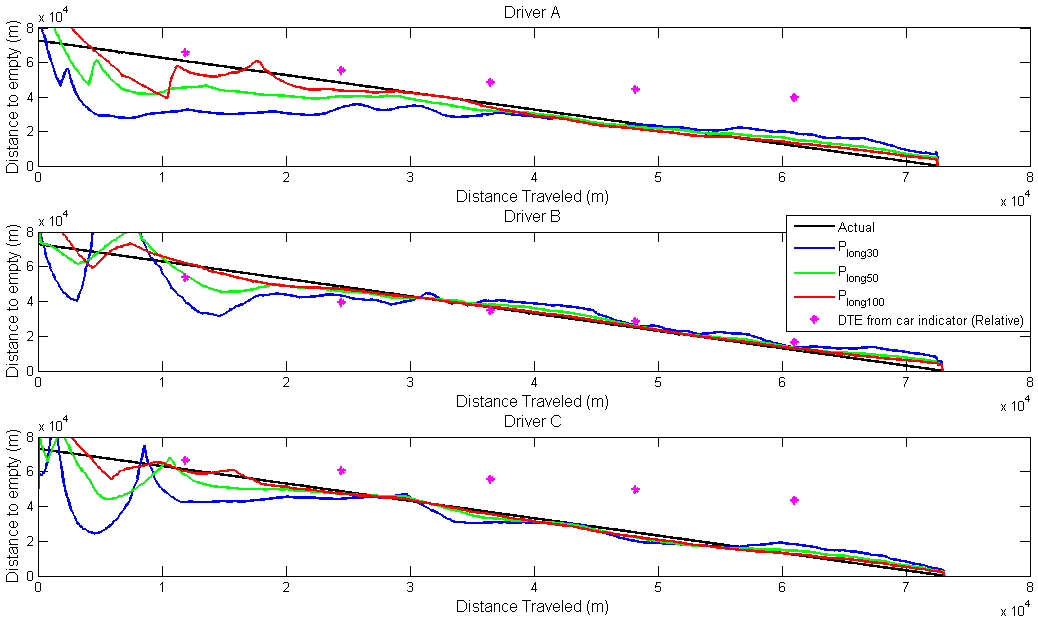
\includegraphics[width=0.5\textwidth]{figs/acmdte}
\caption{\(DTE\) estimated with different-sized terms of fuel intensity (\(p_{long}\)). Red dots are estimates given by in-vehicle displays.}
 \label{fig:dte}
\end{figure}


\begin{table}[!htb]
\label{tab:est}
  \centering
  \begin{tabular}{|c|c|c|c|}
\hline
    Route & Driver A & Driver B & Driver C \\
\hline
\multirow{2}{*}{1} & 1.71 (10.0\%) & 1.23 (17.5\%) & 1.77 (18.8\%)\\
& 1.70 (12.1\%) & 1.18 (19.4\%) & 1.84 (18.6\%)\\
\hline
\multirow{2}{*}{2} & 0.88 (9.6\%) & 0.61 (10.9\%) & 0.81 (22.5\%)
\\
& 0.88 (14.6\%) & 0.59 (22.1\%) & 0.75 (30.7\%)
\\
\hline
\multirow{2}{*}{3} & 0.67 (10.2\%) & 0.57 (7.8\%) & 0.73 (8.7\%)
\\
& 0.65 (4.8\%) & 0.40 (23.2\%) & 0.73 (20.8\%)
\\
\hline
  \end{tabular}
  \caption{Estimation of fuel consumption in litres for each run of each route by each driver, with error in parentheses}
\end{table}

\vspace{-10pt}
\section{Discussion and Future Work} \label{sec:future}

The accuracy of the prediction is limited by the number of training routes, which is in turn limited by the number of drivers. However, the data acquisition system we developed for use in this experiment has been linked to the CloudThink platform \cite{CT:WP:2013}, which is being expanded to include a network of diverse automobile data acquisition devices. Apart from the data gathered by running more experiments of our own, we will be acquiring more data from this platform as its user base expands. More data from more drivers over the same routes, and in different climactic and traffic conditions, will help us address the paucity of data and the short, low-consumption trips in the experiments adversely affecting the accuracy of fuel consumption prediction in this particular demonstration.


{\scriptsize
\bibliographystyle{plain}
\bibliography{reference}
}

\end{document}

